\chapter{Архитектура проекта phantasus}
В этой главе будет рассмотрена архитектура проекта \emph{phantasus}, общая схема, ключевые компоненты и их взаимодействие между ними. Также будут описаны сопутствующие инструменты и их предназначение в системе, и ключевые для архитектуры выдержки из исходного кода.

\section{Общая схема}
Проект \emph{phantasus} состоит из следующих компонент:\begin{itemize}
\item клиентская сторона проекта: \emph{phantasus.js} --- модифицированный \emph{morpheus.js}, дополненный интерфейсами для новых инструментов, поддержкой \texttt{ExpressionSet} и сериализации в \emph{ProtoBuf};
\item серверная сторона проекта: \emph{R}-пакет \emph{phantasus} --- пакет, включающий в себя вычисления и реализации новых инструментов.\end{itemize}

Общую схему взаимодействия можно увидеть на диаграмме~\ref{scheme}.

\begin{figure}[!h]
  \caption{Общая схема проекта \emph{phantasus}}
  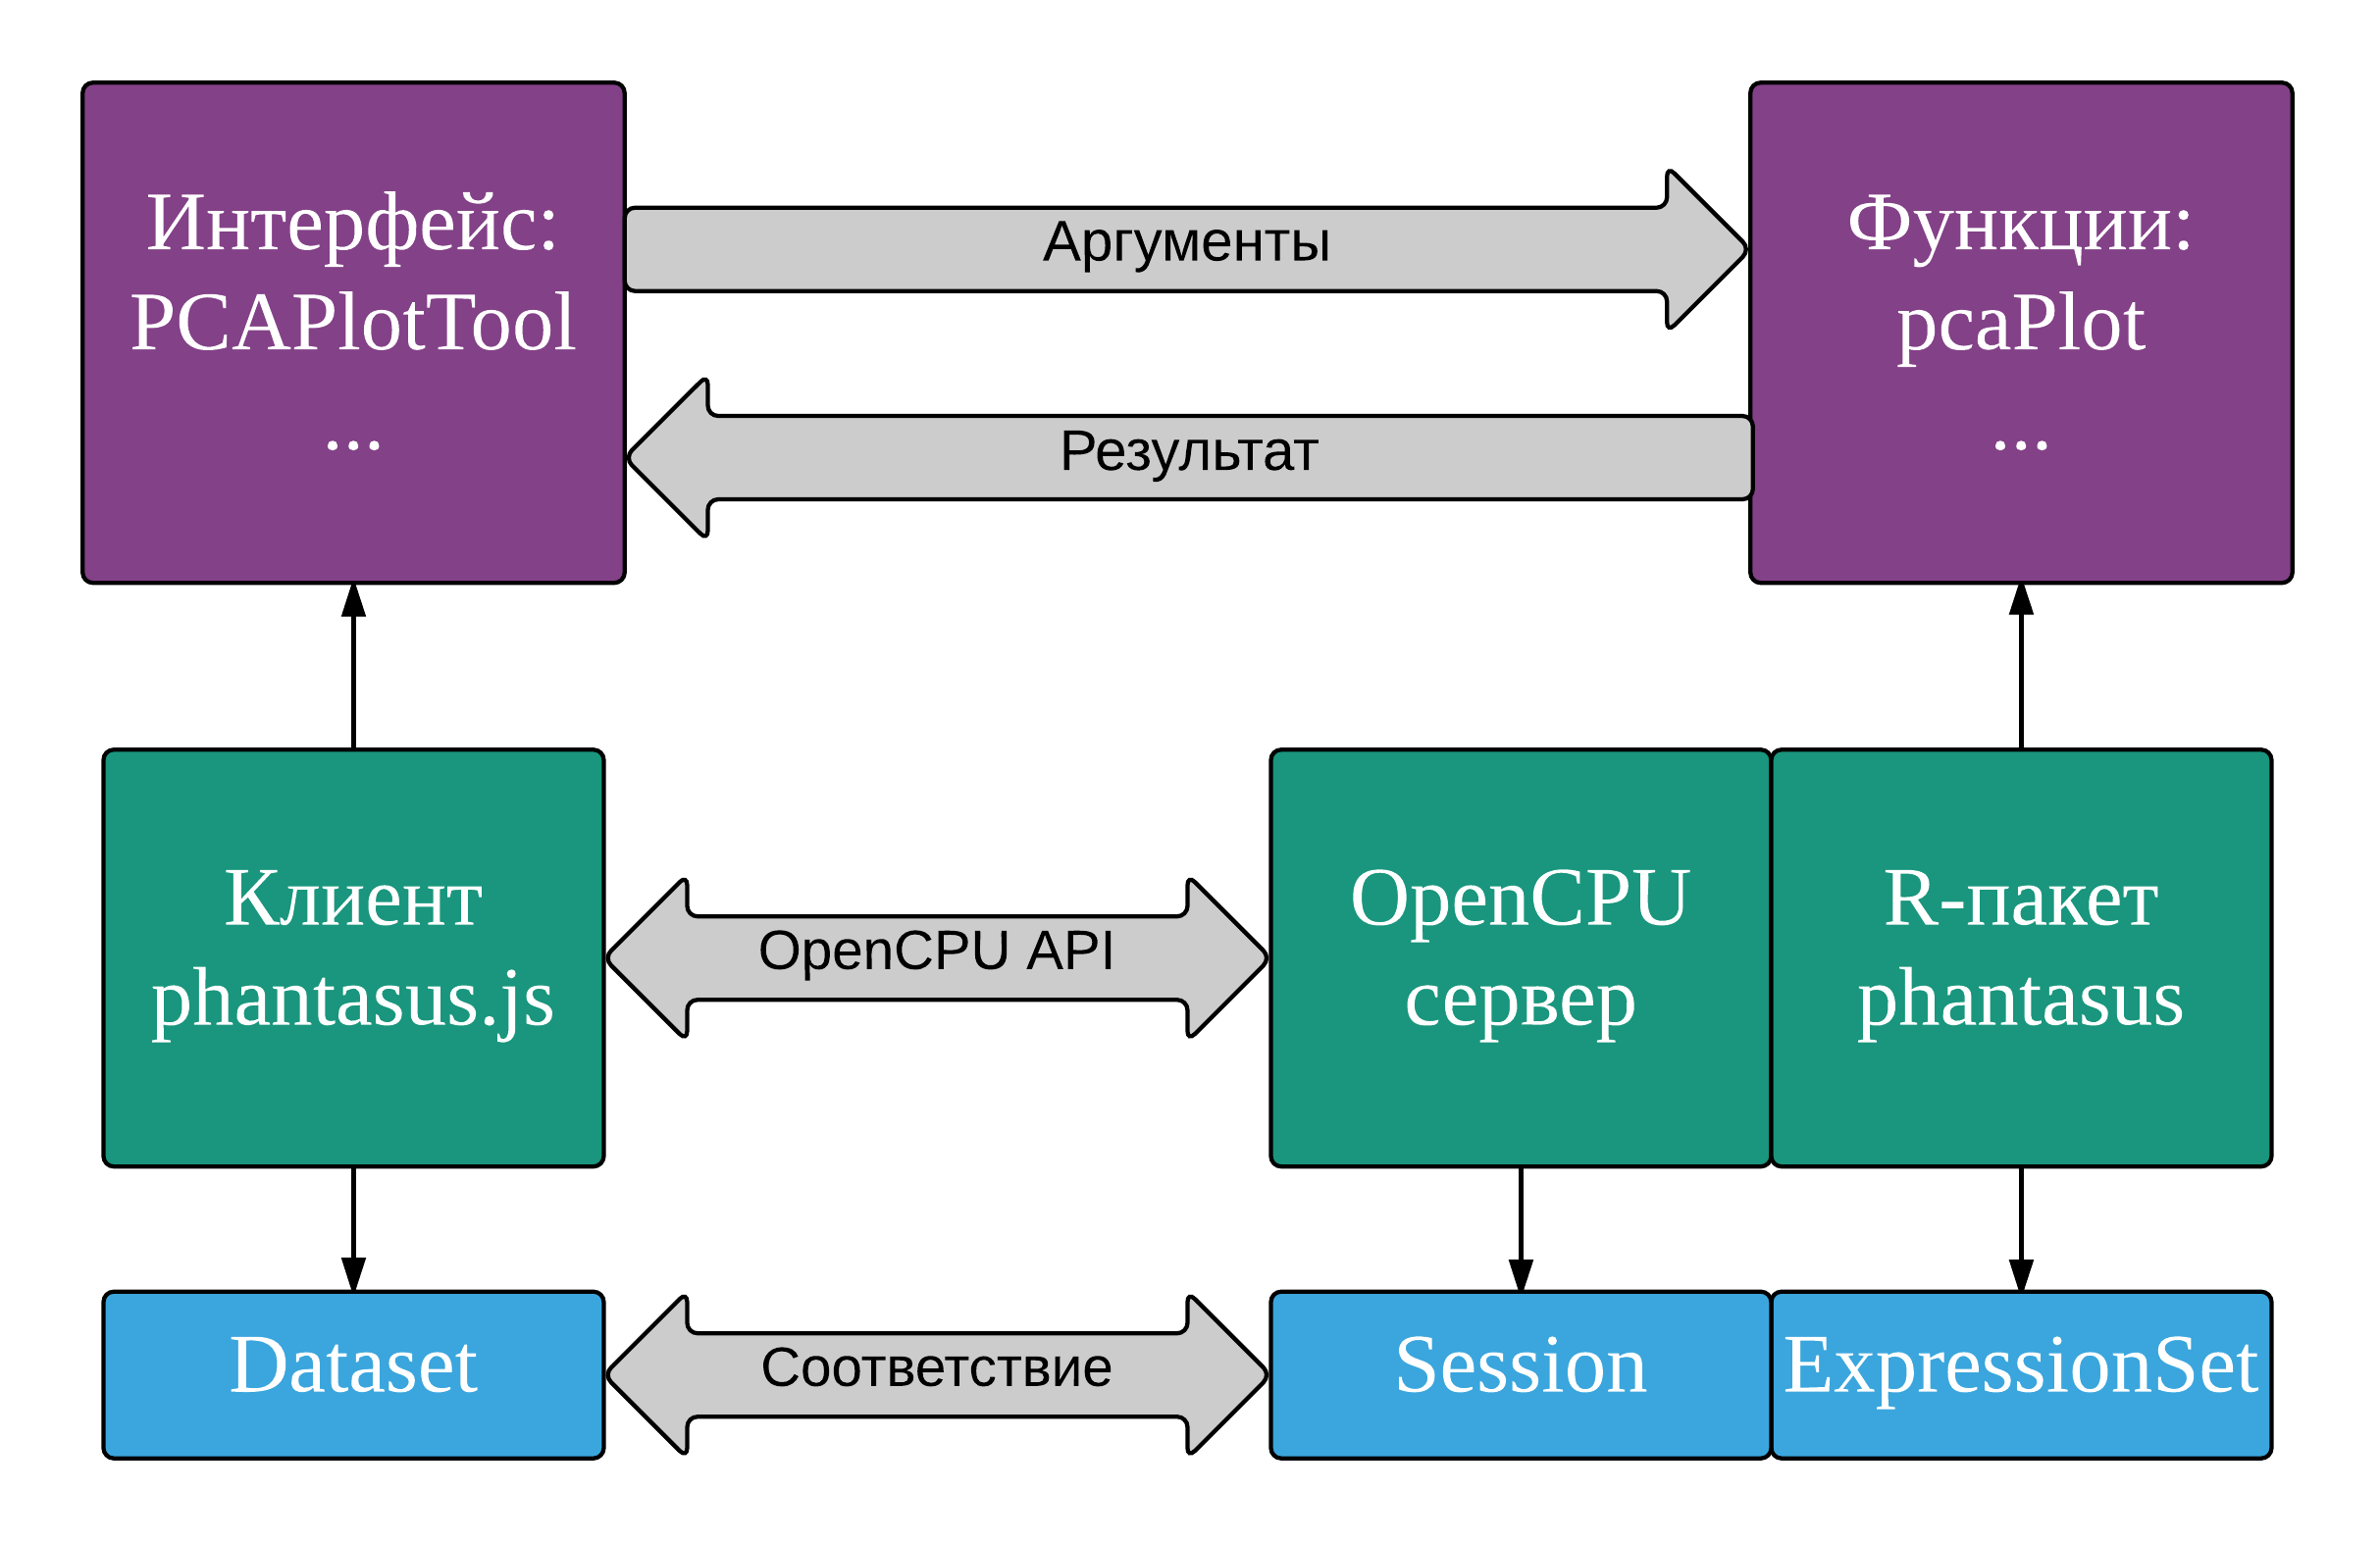
\includegraphics[scale=0.8]{scheme_phantasus.png}
  \label{scheme}
\end{figure}

\section{Взаимодействие между клиентом и сервером}
Все инструменты, реализованные в проекте, имеют две компоненты:\begin{itemize}
\item графический интерфейс в \emph{phantasus.js};
\item вычислительную реализацию в \emph{R}-пакете \emph{phantasus}.
\end{itemize}

Соответственно, для связи этих компонент необходим своеобразный мост между клиентом, написанном на \emph{JavaScript}, и функциями, написанными на \emph{R}. В качестве такого моста используется описанный в обзоре \emph{OpenCPU}.

Помимо наличия моста также необходимо, чтобы общение между клиентом и сервером происходило достаточно быстро, что приводит к потребности в дополнительной сериализации сообщений. В проекте для этого используется протокол \emph{ProtoBuf}.
В данном разделе будет подробно описано об использовании данных технологий при реализации взаимодействия между клиентом и сервером.
\subsection{OpenCPU}
Как было сказано выше, \emph{OpenCPU} используется для связи между \emph{JavaScript}-клиентом и \emph{R}-функциями.

\subsubsection{Использование OpenCPU со стороны клиента}\label{functioncallalgo}
Как было сказано в обзоре, для удобной интеграции \emph{JavaScript} и \emph{R} существует \emph{JavaScript}-библиотека \emph{opencpu.js}, в которой реализованы \emph{RPC}-вызовы. С помощью этой библиотеки в проекте реализована взаимосвязь между графическими интерфейсом инструментов и соответствующих функций из \emph{R}-пакета.

Каждый из инструментов, реализованных в \emph{phantasus.js} действует по следующему принципу:\begin{enumerate}
\item обработка аргументов, полученных в интерфейсе;
\item подготовка данных и аргументов к отправке на сервер;
\item \emph{RPC}-вызов функции, как на листинге~\ref{call.example};
\item обработка содержащегося в полученной сессии результата в виде глобальной переменной, ответа функции или сохраненного в сессии файла;
\item передача ответа в интерфейс.
\end{enumerate}

\subsubsection{Использование OpenCPU со стороны R-пакета}
Со стороны \emph{R}-функций никаким специальным образом не обозначается, что результат работы будет передан именно в \emph{JavaScript}-клиент, все реализованные функции достаточно универсальны.
Функция возвращает результат, в некоторых случаях дополнительно сохраняя его в файл или глобальную переменную, что в дальнейшем использует клиент, который заранее знает, в каком формате получит ответ. 

\subsection{Protocol Buffers}
\emph{OpenCPU API} поддерживает передачу сообщений в \emph{ProtoBuf}-формате. Однако, \emph{JavaScript}-библиотека не предусматривает такой возможности, так что в процессе работы над проектом была добавлена сериализация данных в \emph{ProtoBuf} на стороне клиента и поддержка сериализованных сообщений в \emph{opencpu.js}. 
\subsubsection{Сериализация данных со стороны клиента --- protobuf.js}
Чаще всего обрабатываемые матрицы содержат от 10000 до 40000 строк и от 12 до 40 столбцов. Соответственно, пересылать их между клиентом и сервером в \emph{JSON}-формате слишком долго.

Как было сказано в обзоре, технология \emph{Protocol Buffers} позволяет лучше сериализовать данные, чтобы уменьшить размер пересылаемого пакета.

К сожалению, \emph{Google Developers} официально поддерживают только \emph{Java}, \emph{Python}, \emph{C++}, \emph{Go}, \emph{Objective-C}, \emph{Ruby}, \emph{JavaNano} и \emph{C\#}. Для \emph{JavaScript} сообщество создает поддержку самостоятельно. После анализа существующих решений, было решено выбрать библиотеку \emph{ProtoBuf.js}~\cite{protobufjs}.

Данная библиотека реализует класс \texttt{Builder}, который компилируется из \texttt{*.proto}-файлов и позволяет получить доступ к сериализованным данным. С помощью экземпляра данного класса можно закодировать соответствующий \emph{JSON}-объект в \texttt{Uint8Array}, чтобы после переслать его в сжатом виде на сервер.

Для преобразования экземпляров классов \texttt{Dataset} и \texttt{SlicedDatasetView}, которые были представлены в обзоре приложения \emph{morpheus.js}, в сериализованнный \texttt{Uint8Array} используется протокол, описанный в приложении~\ref{proto}. Данный протокол используется также в \emph{R}-пакете \emph{protolite}~\cite{protolite}, с помощью которого данные десериализуются на сервере.

Таким образом в класс \texttt{DatasetUtil} была добавлена утилита, сериализующая \texttt{Dataset}, которая используется перед отправкой данных на сервер, и десериализующая результат работы \emph{R}-функций, если те сохраняют результат в бинарном файле. 
\subsubsection{Сериализация данных со стороны сервера --- protolite}
Внутри \emph{R}-функций нет необходимости вручную явно десериализовавать входные данные, так как \emph{OpenCPU} автоматически разбирает аргументы до входа в функцию.

Однако, если функция возвращает матрицы больших размеров, используется \emph{R}-пакет \emph{protolite}~\cite{protolite} для сериализации результата работы, который после сериализованный записывается в бинарный файл. В дальнейшем этот файл считывается клиентом из директории возвращенной временной сессии. 

\section{Поддержка ExpressionSet}
Как было сказано ранее, а также продемонстрировано на схеме~\ref{scheme}, в ходе работы приложения постоянно поддерживается соответствие между экземпляром класса \texttt{Dataset} на клиенте и экземпляром класса \texttt{ExpressionSet} на сервере. В данном разделе будет подробнее разобрана реализация данного соответствие.
\subsection{Поддержка ExpressionSet на стороне клиента}
В \emph{phantasus.js} в Dataset добавлено дополнительное поле \texttt{esSession}, в котором находится объект класса \texttt{Promise} для асинхронного обновления ключа сессии в этом поле.

При загрузке или обновлении \texttt{Dataset} осуществляется следующий ряд действий:
\begin{enumerate}
\item в поле \texttt{dataset.esSession} записывается экземпляр класса \texttt{Promise}, который позволяет продолжать загрузку данных в фоновом режиме, а также ждать, когда данные будут обработаны прежде чем запускать функции использующие \texttt{ExpressionSet} в качестве аргумента (\texttt{pcaPlot}, \texttt{kmeans}, \texttt{limma}). При создании \texttt{Promise} в аргументах указывается две функции: \texttt{reject} и \texttt{resolve};
\item актуальное содержимое экземпляра класса \texttt{Dataset} вместе с матрицей и аннотацией сериализуется в \emph{ProtoBuf} по протоколу, описанному в приложении~\ref{proto};
\item с помощью \emph{opencpu.js} отправляется \emph{RPC} за функцией \texttt{createES} с аргументом в виде сериализованных данных;
\item данные поступают на сервер, десериализуются там автоматически и функция \texttt{createES} создает \texttt{ExpressionSet}, являющийся копией \texttt{Dataset} из клиента;
\item функция \texttt{createES} объявляет данный \texttt{ExpressionSet} глобальной переменной, таким образом имеется доступ к этому объекту по \emph{API-entrypoint} \texttt{/ocpu/tmp/{key}/R/es};
\item по завершении \emph{RPC} получает ключ временной сессии, содержащий созданный \texttt{ExpressionSet} и завершает \texttt{Promise} с \texttt{resolve(session)};
\item если во время одного из этапов произошла ошибка, то \texttt{Promise} завершается с \texttt{reject(error)} с текстом ошибки.
\end{enumerate}

\subsection{Создание ExpressionSet из внешних данных на стороне сервера} \label{createESsection}
В начале работы с \emph{phantasus} необходимо загрузить данные. Если данные загружены из файла, то они будут сначала обработаны на клиенте, а после пересланы на сервер для создания \emph{ExpressionSet} из них с помощью кода на листинге~\ref{createES}.

Функция \texttt{createES} принимает следующие аргументы:\begin{itemize}
\item \texttt{data} --- непосредственно матрица экспрессии;
\item \texttt{pData} --- аннотация к образцам;
\item \texttt{varLabels} --- названия характеристик описания образцов;
\item \texttt{fData} --- аннотация к генам;
\item \texttt{fvarLabels} --- названия характеристик описания генов.
\end{itemize}

\begin{lstlisting}[float=!h,caption={Функция создания ExpressionSet из исходных данных},label={createES},language=R]
createES <- function(data, pData, varLabels, fData, fvarLabels) {
  exprs <- t(data)
  phenoData <- AnnotatedDataFrame(data.frame(pData))
  varLabels(phenoData) <- varLabels
  
  featureData <- AnnotatedDataFrame(data.frame(fData))
  varLabels(featureData) <- fvarLabels
 
  es <- ExpressionSet(assayData = exprs, phenoData=phenoData, featureData = featureData)
  assign("es", es, envir = parent.frame())
  es
}
\end{lstlisting}

По завершении функция отправляет \texttt{es} в глобальные переменные, чтобы созданный \texttt{ExpressionSet} был доступен по адресу: \texttt{/ocpu/tmp/{key}/R/es}. Таким образом, получив ключ данной сессии, можно иметь доступ и к \texttt{ExpressionSet}, находящемуся в ней.

Ключ сессии обновляется каждый раз при изменении \texttt{Dataset} в \emph{phantasus.js}. Чаще всего изменения происходят в результате работы одного из следующих инструментов: \texttt{Adjust}, \texttt{Collapse}, \texttt{new HeatMap}, \texttt{Transpose}. Изменные данные, точно так же ,как и новые, пересылаются на сервер и ключ сессии обновляется в поле \texttt{esSession} в \texttt{Dataset}.

\section{Способы визуализации}
В данном разделе будут показаны достоинства и недостатки различных способов визуализации, а также применимость в различных ситуациях. 
\subsection{Отрисовка графиков на стороне сервера}
Первый вариант визуализации графиков и схем состоит в отрисовке их там же, где и происходит вычисление всех необходимых для них данных, то есть на сервере внутри \emph{R}-функции. Данный способ подразумевает отрисовку и сохранение изображений в виде \emph{png} или \emph{svg}-файла, который сохраняется внутри временной \emph{OpenCPU}-сессии. Клиент после забирает из сессии изображение и показывает в графическом интерфейсе приложения.

Достойнства:\begin{itemize}
\item возможность пользоваться проверенными \emph{R}-пакетами для визуализации, например, \emph{ggplot2}~\cite{ggplot2};
\item файл можно переиспользовать при необходимости, нужно знать только ключ сессии, где он находится.
\end{itemize}

Однако таким образом можно использовать только статичные изображения.

\subsection{Визуализация на стороне клиента}
Для отображения интерактивных графиков удобно использовать библиотеку \emph{plotly.js}~\cite{plotly}, которая предоставляет \emph{API}, где описание графика строится в \emph{JSON}-формате.
Таким образом можно строить интерактивные изображения, переложить всю работу по визуализации с сервера на клиент.

Именно этот способ на данный момент используется в проекте, подробнее об инструменте будет рассказано в главе~\ref{implementation}.

\chapterconclusion
В данной главе были рассмотрены основные составляющие проекта:
\begin{itemize}
\item \emph{phantasus.js} --- расширенный \emph{morpheus.js};
\item \emph{R}-пакет \emph{phantasus} --- \emph{R}-пакет, содержащий в себе серверные реализации всех добавленных методов и инструментов.
\end{itemize}

Также были представлены следующие подробности архитектуры проекта:\begin{itemize}
\item общая схема всего проекта, где показаны компоненты и связи между ними;
\item способ взаимодействия между компонентами с помощью \emph{OpenCPU};
\item сериализация данных в \emph{ProtoBuf} на стороне клиента и на стороне сервера;
\item поддержка \texttt{ExpressionSet};
\item способы визуализации.
\end{itemize}
